\section{AI Agent Layer}

\begin{frame}
    \frametitle{Components}
    \begin{figure}
        \centering
        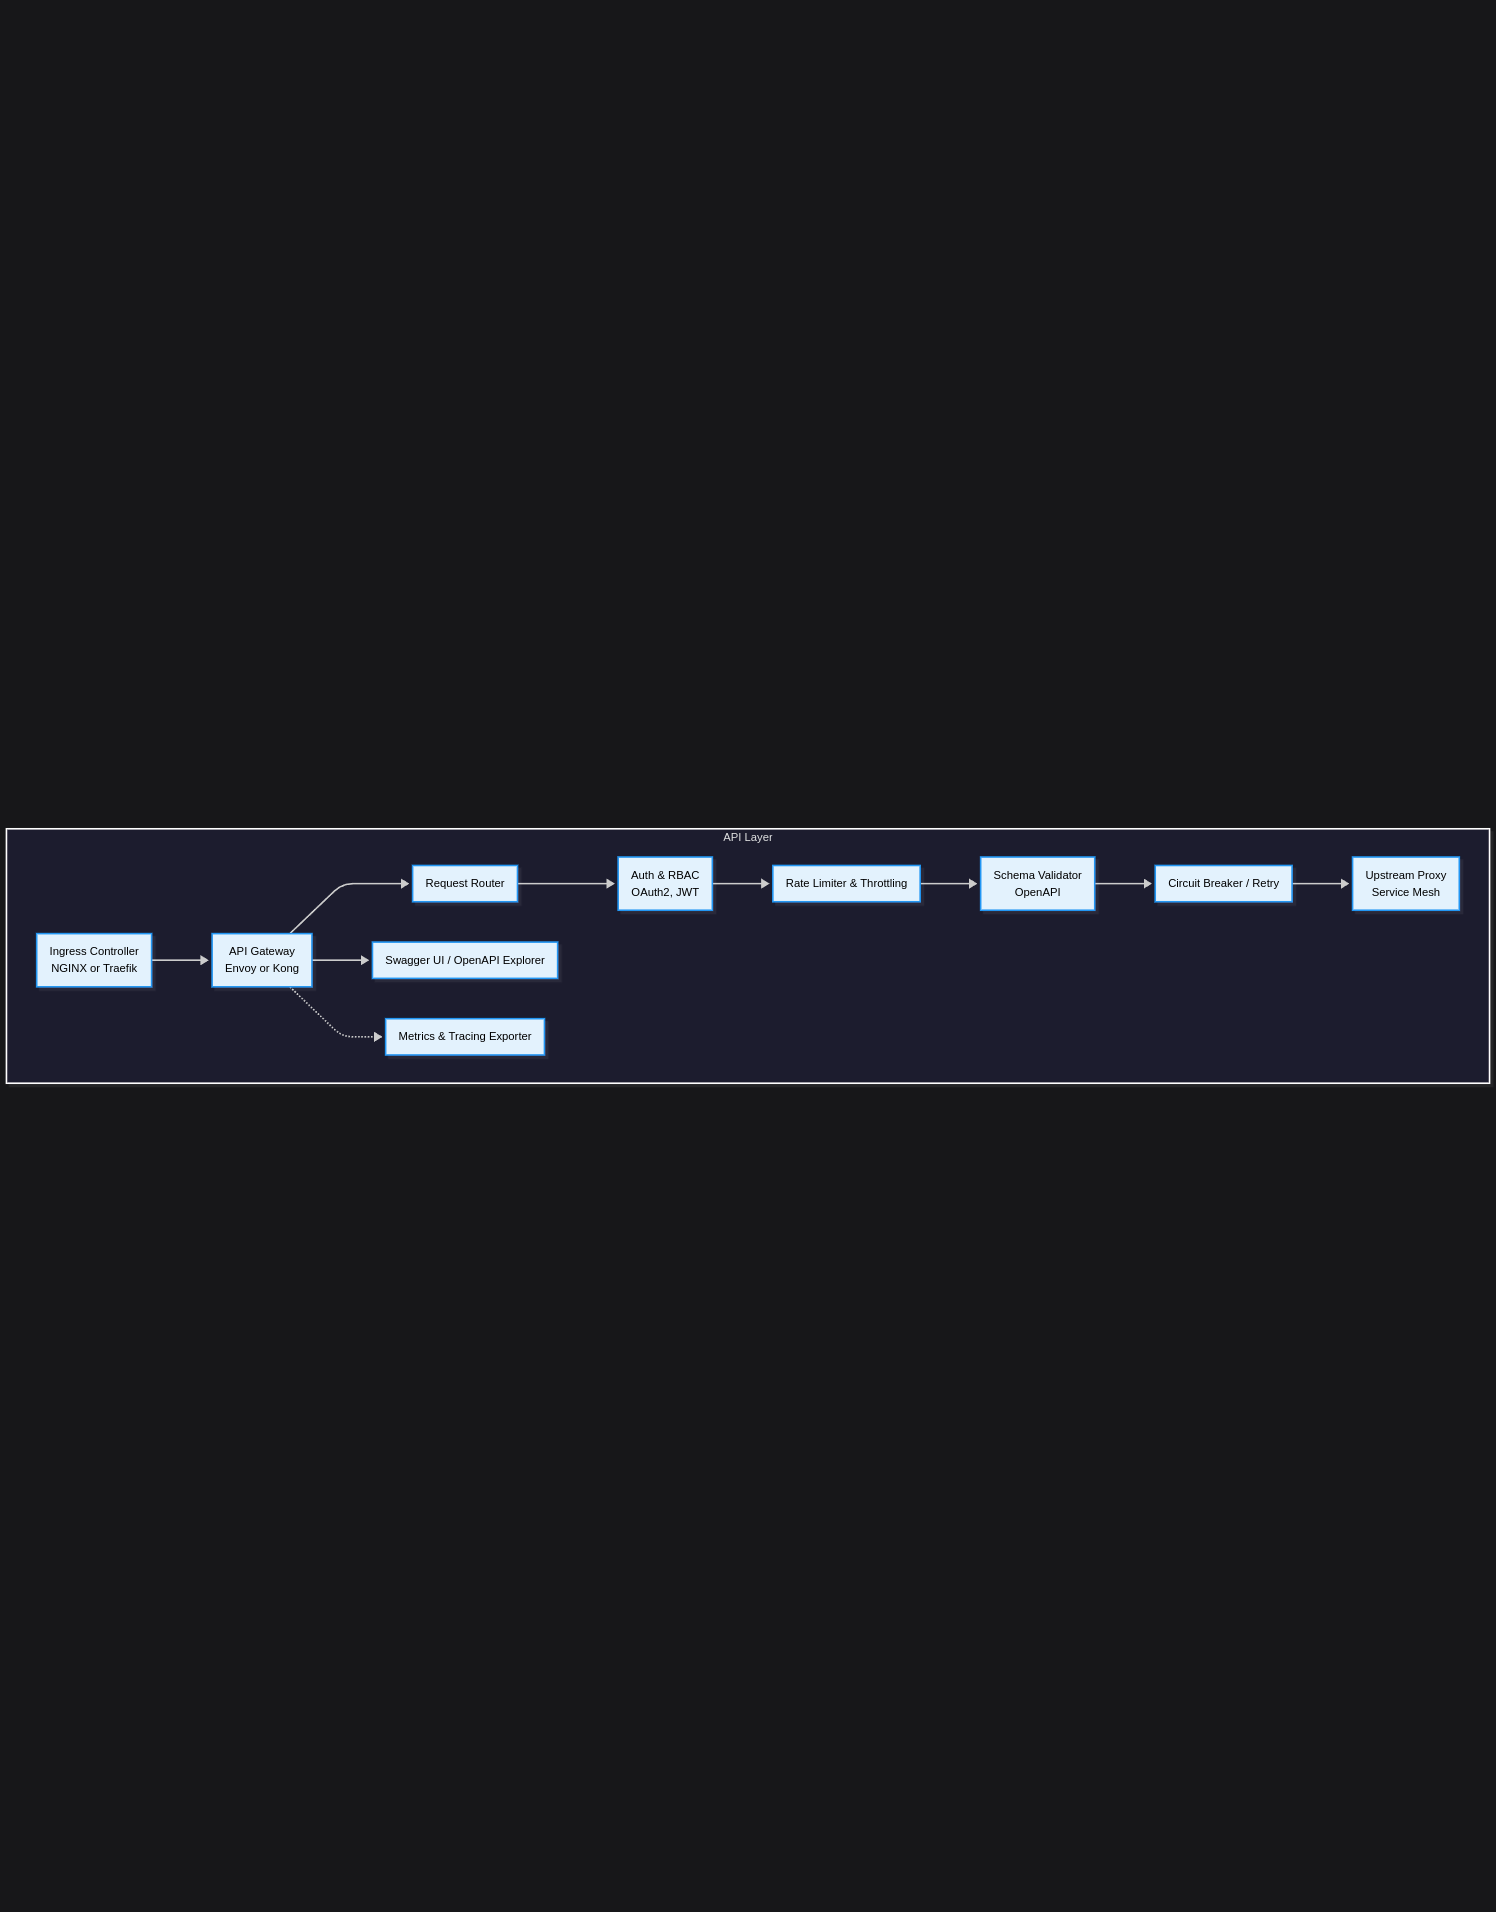
\includegraphics[width=0.3\textwidth]{ai/layout.png} % Adjusted the scale of the image to 0.5
        \caption{ Layer Layout}
    \end{figure}
\end{frame}

\begin{frame}
    \frametitle{ Sequence Flow}
    \begin{figure}
        \centering
        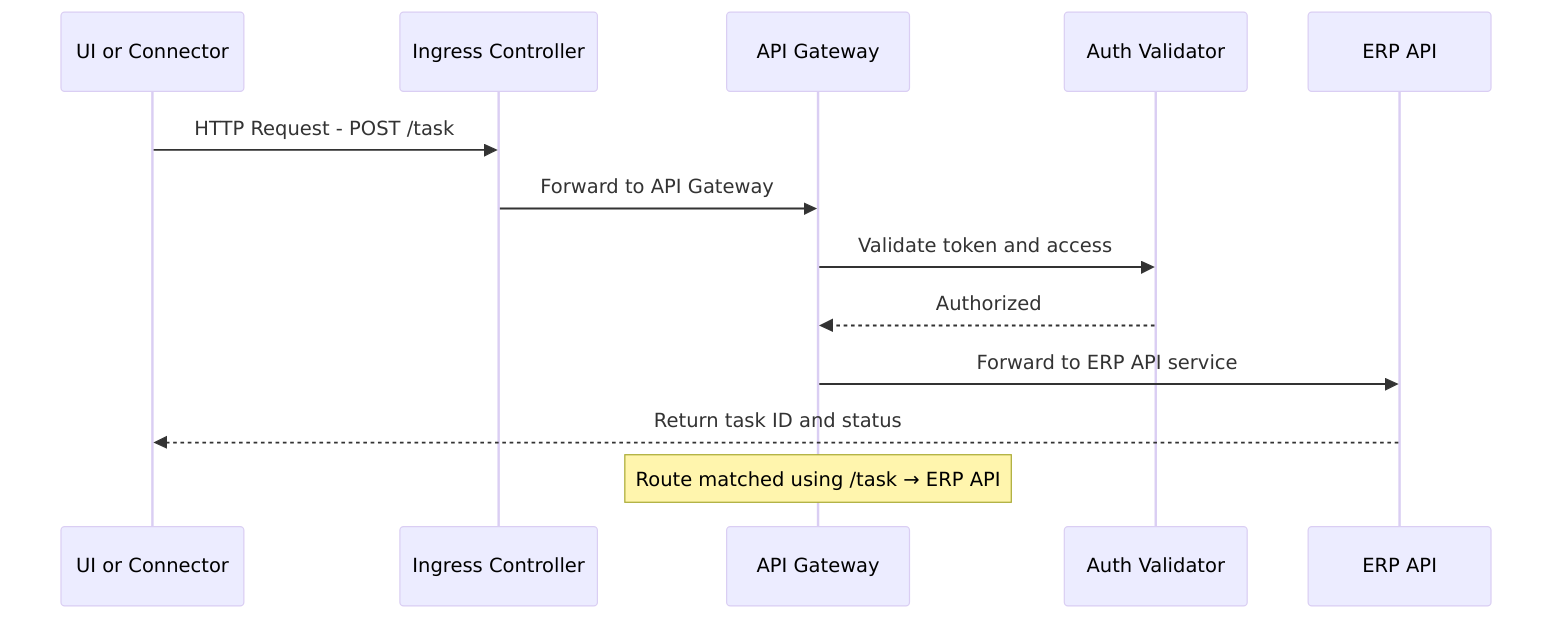
\includegraphics[width=0.8\textwidth]{ai/sequence.png} % Adjusted the scale of the image to 0.5
        \caption{ Sequence Flow}
    \end{figure}
\end{frame}



% Dividing the first table into multiple frames with 5 or 6 rows each
\begin{frame}
    \frametitle{AI Agent Layer - Functional Responsibilities (Part 1)}
    \begin{itemize}
        \item \textbf{Email Agent}: Parse instructions, project context, and intent from incoming emails.
        \item \textbf{Doc Extraction Agent}: Extract data from tables, forms, and scanned docs using OCR or layout models.
        \item \textbf{Document Generation Agent}: Generate structured documents like BoQ or datasheets from extracted data.
        \item \textbf{Compliance Agent}: Validate content against standards, checklists, and tender specs.
        \item \textbf{Diagram GPT}: Parse and understand flow diagrams like P and ID or layout maps.
        \item \textbf{ERP Action Agent}: Convert natural language into ERP commands or task state changes.
    \end{itemize}
\end{frame}

\begin{frame}
    \frametitle{AI Agent Layer - Functional Responsibilities (Part 2)}
    \begin{itemize}
        \item \textbf{Project Query Agent}: Answer task-related queries across agents and document context.
        \item \textbf{Enquiry Agent}: Parse RFQs to extract delivery dates, quantities, vendor details.
        \item \textbf{AI Review Summary Agent}: Generate summaries for human reviewers with context awareness.
        \item \textbf{Semantic Diff Agent}: Highlight structural and content changes between document versions.
        \item \textbf{Iteration Summary Agent}: Track changes over task lifecycle and report rejections, updates.
        \item \textbf{Change Justification Agent}: Prompt reviewer to explain rejection or suggest revision reason.
    \end{itemize}
\end{frame}

% % Dividing the second table into multiple frames with 5 or 6 rows each
% \begin{frame}
%     \frametitle{AI Agent Layer - Technical Responsibilities (Part 1)}
%     \begin{table}[h!]
% \centering
% \renewcommand{\arraystretch}{1.2}
% \begin{tabular}{|p{3cm}|p{7cm}|}
% \hline
% \textbf{Agent Name} & \textbf{Technical Responsibility} \\
% \hline
% Email Agent & NLP pipeline with rule-based intent parser, optionally tied to email gateway or ERP API \\
% \hline
% Doc Extraction Agent & Uses OCR or layout parser for tables and text zones, outputs structured fields \\
% \hline
% Document Generation Agent & Template-to-prompt pipeline with slot filling, LLM-based output generation \\
% \hline
% Compliance Agent & Rule engine and prompt chain for checklist validation and clause comparison \\
% \hline
% Diagram GPT & VLM (e.g. Layout Parser + LLM) to parse nodes, connections, and symbols \\
% \hline
% ERP Action Agent & Prompt-tuned agent that maps instructions to ERP APIs or state updates \\
% \hline
% \end{tabular}
% \caption{AI Agent Layer - Technical Responsibilities (Part 1)}
% \end{table}
% \end{frame}

% \begin{frame}
%     \frametitle{AI Agent Layer - Technical Responsibilities (Part 2)}
%     \begin{table}[h!]
% \centering
% \renewcommand{\arraystretch}{1.2}
% \begin{tabular}{|p{3cm}|p{7cm}|}
% \hline
% \textbf{Agent Name} & \textbf{Technical Responsibility} \\
% \hline
% Project Query Agent & Uses vector or structured context store to resolve task or project questions \\
% \hline
% Enquiry Agent & Uses prompt chaining to extract quantities, specs, RFQ tables, and requirements \\
% \hline
% AI Review Summary Agent & Extracts section highlights and generates human-reviewable summaries \\
% \hline
% Semantic Diff Agent & Compares two files via structure, token diff, and summary generation \\
% \hline
% Iteration Summary Agent & Aggregates change history and task metadata to summarize evolution \\
% \hline
% Change Justification Agent & Prompts reviewers for structured or free-form explanation, logs it to task \\
% \hline
% \end{tabular}
% \caption{AI Agent Layer - Technical Responsibilities (Part 2)}
% \end{table}
% \end{frame}

